\documentclass{standalone}
\usepackage{tikz}
\usetikzlibrary{patterns}
\usetikzlibrary{positioning}
\usetikzlibrary{patterns, positioning}
\usetikzlibrary{shapes.misc}
\usepackage[outline]{contour}
\contourlength{1.5pt} 


\begin{document}
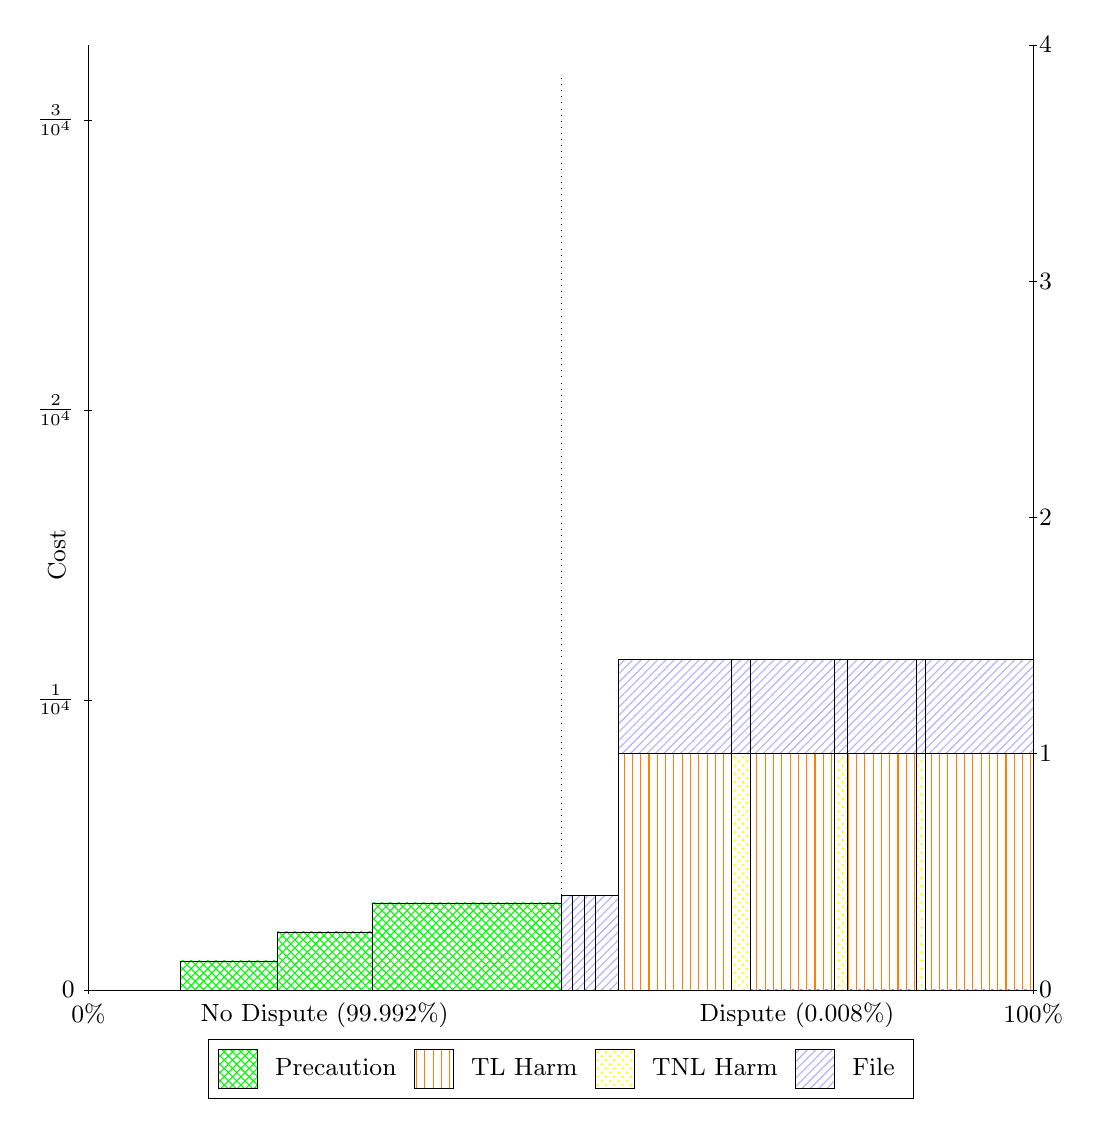
\begin{tikzpicture}
\draw[pattern=crosshatch, pattern color=green,draw=black,very thin] (2.6643,2.5) rectangle (3.8994,2.8682);
\draw[pattern=crosshatch, pattern color=green,draw=black,very thin] (3.8994,2.5) rectangle (5.1005,3.2363);
\draw[pattern=crosshatch, pattern color=green,draw=black,very thin] (5.1005,2.5) rectangle (7.5,3.6045);
\draw[pattern=north east lines, pattern color=blue!30,draw=black,very thin] (7.5,2.5) rectangle (7.6429,3.7);
\draw[pattern=crosshatch, pattern color=green,draw=black,very thin] (7.6429,2.5) rectangle (7.7945,2.5);
\draw[pattern=north east lines, pattern color=blue!30,draw=black,very thin] (7.6429,2.5) rectangle (7.7945,3.7);
\draw[pattern=crosshatch, pattern color=green,draw=black,very thin] (7.7945,2.5) rectangle (7.9419,2.5001);
\draw[pattern=north east lines, pattern color=blue!30,draw=black,very thin] (7.7945,2.5001) rectangle (7.9419,3.7001);
\draw[pattern=crosshatch, pattern color=green,draw=black,very thin] (7.9419,2.5) rectangle (8.2363,2.5001);
\draw[pattern=north east lines, pattern color=blue!30,draw=black,very thin] (7.9419,2.5001) rectangle (8.2363,3.7001);
\draw[pattern=vertical lines, pattern color=orange,draw=black,very thin] (8.2363,2.5) rectangle (9.6654,5.5);
\draw[pattern=north east lines, pattern color=blue!30,draw=black,very thin] (8.2363,5.5) rectangle (9.6654,6.7);
\draw[pattern=crosshatch, pattern color=green,draw=black,very thin] (9.6654,2.5) rectangle (9.9039,2.5);
\draw[pattern=crosshatch dots, pattern color=yellow,draw=black,very thin] (9.6654,2.5) rectangle (9.9039,5.5);
\draw[pattern=north east lines, pattern color=blue!30,draw=black,very thin] (9.6654,5.5) rectangle (9.9039,6.7);
\draw[pattern=crosshatch, pattern color=green,draw=black,very thin] (9.9039,2.5) rectangle (10.979,2.5);
\draw[pattern=vertical lines, pattern color=orange,draw=black,very thin] (9.9039,2.5) rectangle (10.979,5.5);
\draw[pattern=north east lines, pattern color=blue!30,draw=black,very thin] (9.9039,5.5) rectangle (10.979,6.7);
\draw[pattern=crosshatch, pattern color=green,draw=black,very thin] (10.979,2.5) rectangle (11.137,2.5001);
\draw[pattern=crosshatch dots, pattern color=yellow,draw=black,very thin] (10.979,2.5001) rectangle (11.137,5.5001);
\draw[pattern=north east lines, pattern color=blue!30,draw=black,very thin] (10.979,5.5001) rectangle (11.137,6.7001);
\draw[pattern=crosshatch, pattern color=green,draw=black,very thin] (11.137,2.5) rectangle (12.019,2.5001);
\draw[pattern=vertical lines, pattern color=orange,draw=black,very thin] (11.137,2.5001) rectangle (12.019,5.5001);
\draw[pattern=north east lines, pattern color=blue!30,draw=black,very thin] (11.137,5.5001) rectangle (12.019,6.7001);
\draw[pattern=crosshatch, pattern color=green,draw=black,very thin] (12.019,2.5) rectangle (12.124,2.5001);
\draw[pattern=crosshatch dots, pattern color=yellow,draw=black,very thin] (12.019,2.5001) rectangle (12.124,5.5001);
\draw[pattern=north east lines, pattern color=blue!30,draw=black,very thin] (12.019,5.5001) rectangle (12.124,6.7001);
\draw[pattern=crosshatch, pattern color=green,draw=black,very thin] (12.124,2.5) rectangle (13.5,2.5001);
\draw[pattern=vertical lines, pattern color=orange,draw=black,very thin] (12.124,2.5001) rectangle (13.5,5.5001);
\draw[pattern=north east lines, pattern color=blue!30,draw=black,very thin] (12.124,5.5001) rectangle (13.5,6.7001);
\draw[black,very thin] (1.5,2.5) -- (1.5,14.5);
\node[font=\small,rotate=90,text=black, anchor=center] at (1.1, 8.0226) {Cost};
\draw[black,very thin] (1.45,2.5) -- (1.55,2.5);
\node[font=\small,text=black, anchor=east] at (1.45, 2.5) {0};
\draw[black,very thin] (1.45,6.1817) -- (1.55,6.1817);
\node[font=\small,text=black, anchor=east] at (1.45, 6.1817) {$\frac{1}{10^{4}}$};
\draw[black,very thin] (1.45,9.8634) -- (1.55,9.8634);
\node[font=\small,text=black, anchor=east] at (1.45, 9.8634) {$\frac{2}{10^{4}}$};
\draw[black,very thin] (1.45,13.545) -- (1.55,13.545);
\node[font=\small,text=black, anchor=east] at (1.45, 13.545) {$\frac{3}{10^{4}}$};

\draw[black,dotted,very thin] (7.5,2.86) -- (7.5,14.14);
\draw[black,very thin] (13.5,2.5) -- (13.5,14.5);
\draw[black,very thin] (13.45,2.5) -- (13.55,2.5);
\node[font=\small,text=black, anchor=west] at (13.45, 2.5) {0};
\draw[black,very thin] (13.45,5.5) -- (13.55,5.5);
\node[font=\small,text=black, anchor=west] at (13.45, 5.5) {1};
\draw[black,very thin] (13.45,8.5) -- (13.55,8.5);
\node[font=\small,text=black, anchor=west] at (13.45, 8.5) {2};
\draw[black,very thin] (13.45,11.5) -- (13.55,11.5);
\node[font=\small,text=black, anchor=west] at (13.45, 11.5) {3};
\draw[black,very thin] (13.45,14.5) -- (13.55,14.5);
\node[font=\small,text=black, anchor=west] at (13.45, 14.5) {4};

\draw[black,very thin] (1.5,2.5) -- (13.5,2.5);
\draw[black,very thin] (1.5,2.45) -- (1.5,2.55);
\node[font=\small,text=black, anchor=north] at (1.5, 2.45) {0\%};
\draw[black,very thin] (13.5,2.45) -- (13.5,2.55);
\node[font=\small,text=black, anchor=north] at (13.5, 2.45) {100\%};

\node[font=\small,text=black,anchor=south] at (4.5, 1.9) {No\ Dispute\ (99.992\%)};
\node[font=\small,text=black,anchor=south] at (10.5, 1.9) {Dispute\ (0.008\%)};
\draw (7.5,2.5) node (B) {};
\begin{scope}[align=center]
\matrix[scale=0.5,draw=black,below=0.5cm of B,nodes={draw},column sep=0.1cm]{
\node[rectangle,draw,minimum width=0.5cm,minimum height=0.5cm,pattern=crosshatch, pattern color=green]{}; & \node[draw=none,font=\small,text=black]{Precaution}; &
\node[rectangle,draw,minimum width=0.5cm,minimum height=0.5cm,pattern=vertical lines, pattern color=orange]{}; & \node[draw=none,font=\small,text=black]{TL Harm}; &
\node[rectangle,draw,minimum width=0.5cm,minimum height=0.5cm,pattern=crosshatch dots, pattern color=yellow]{}; & \node[draw=none,font=\small,text=black]{TNL Harm}; &
\node[rectangle,draw,minimum width=0.5cm,minimum height=0.5cm,pattern=north east lines, pattern color=blue!30]{}; & \node[draw=none,font=\small,text=black]{File}; \\\\
};\end{scope}

\end{tikzpicture}
\end{document}